\newpage
\subsection{Needfinding}
Needfinding is the process of discovering what users \textit{need}, not what they \textit{want}.
This is an important distinction, because most users can't actually tell you what they want unless presented with multiple options to choose from.

While it is a good idea to talk to users about what they are annoyed with in the system, asking them how they would change it is likely not going to give you much of an idea
as to what you should change. Instead envision what could be possible solutions to the issues the users mentioned and implement mock-ups or prototypes for some of them and
give those to actual users to try out, mentioning of course that this not a finished product.

This brings us to the distinction between {\color{red} \textit{Needs}} (human goals, i.e. what a user needs to achieve their task),
{\color{ForestGreen} \textit{Requirements}} (system goals, i.e. what the system needs to accomplish)
and {\color{Blue} \textit{Features}} (solutions to the goals, but are not requirements by themselves).

Thus it is important to find out \textit{why} the user does something in a certain way and \textit{how} the user wants something and we know that we are doing the right thing.

\subsubsection{Why}
To find out why users do things a certain way is to ask basic questions of everyday experiences, but don't do that with closed-ended questions,
such as ``Do you like this design'', and instead use something like ``What do you like about the design and what would you like changed?''.
Remember to not ask \textit{how} they want it changed, because that's not something users typically are good at.

\subsubsection{How}
How do we know if we are asking the right questions and if asking questions is even enough?
Furthermore, two different people may interpret the same answers differently.

And finally, there are various biases:
\begin{itemize}
    \item \bi{Confirmation Bias}: The human brain tends to only consider facts that confirm ones view
    \item \bi{Sampling Bias}: It is rarely possible to get a representative sample of all the users,
          which means that you will typically only get the opinions of the users that are easiest to reach.
    \item \bi{Good Participant Bias}: Users tend to try to give positive or acceptable answers to please the researchers.
    \item \bi{Hypothetical Bias}: Some users may say they would use a feature (in a certain way), but when actually having to use it, they won't.
    \item \bi{Recency Bias}: Users focus on the most recent experience
    \item \bi{Groupthink}: Design teams align too quickly on an interpretation without challenging it.
\end{itemize}
Common needfinding methods include:
\begin{multicols}{3}
    \begin{itemize}
        \item Interview
        \item Diary Study
        \item Retrospective Study
        \item Artifact Analysis
        \item Contextual Inquiry
    \end{itemize}
\end{multicols}

\subsubsection{Five Stages of Design Thinking}
\begin{center}
    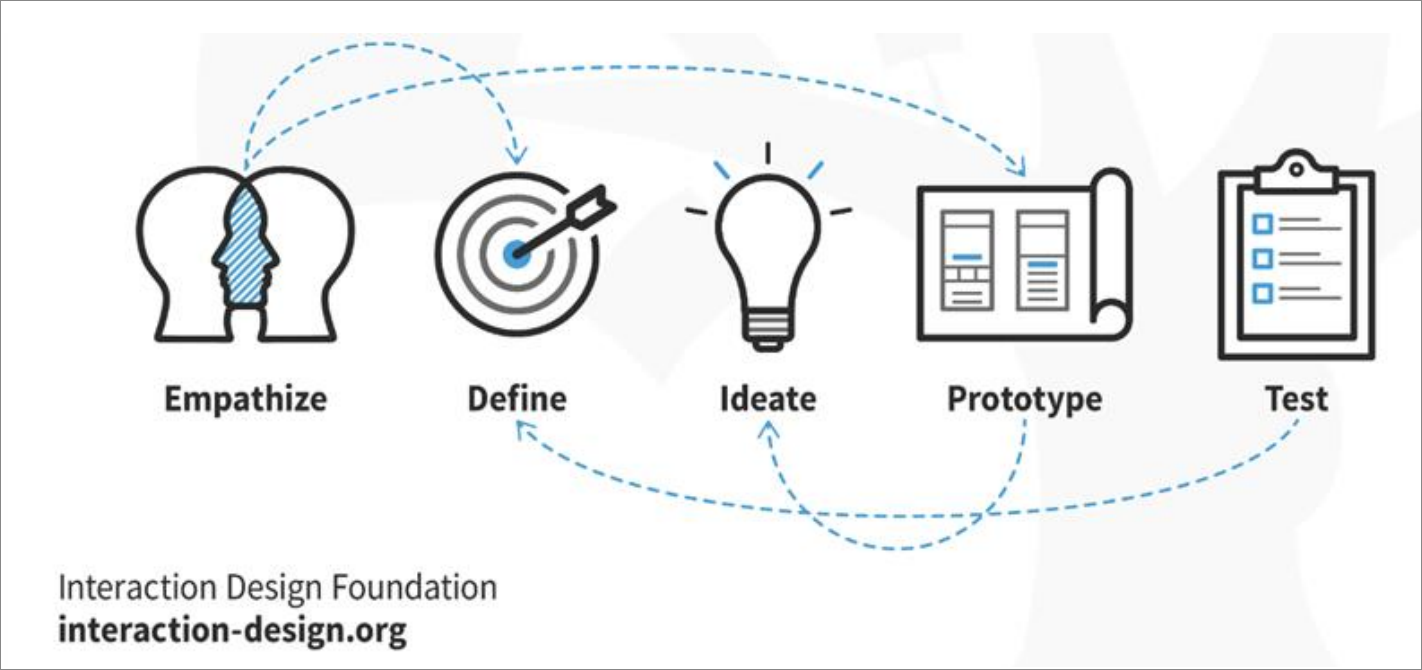
\includegraphics[width=0.7\linewidth]{assets/design-thinking.png}
\end{center}
